\documentclass[aspectratio=169]{beamer}
\usetheme{Madrid}
\usecolortheme{default}
\usepackage{booktabs}
\usepackage{amsmath}
\usepackage{graphicx}
\graphicspath{{presentation/figures/}{figures/}}
\usepackage{xcolor}
\usepackage{tikz}
\usepackage{multirow}
\AtBeginEnvironment{frame}{\tiny}

% ---- Custom Colors ----
\definecolor{rungblue}{RGB}{31, 119, 180}
\definecolor{rungorange}{RGB}{255, 127, 14}
\definecolor{runggreen}{RGB}{44, 160, 44}
\definecolor{darkblue}{RGB}{0, 51, 102}

\setbeamercolor{frametitle}{bg=darkblue, fg=white}
\setbeamercolor{title}{bg=darkblue, fg=white}
\setbeamercolor{block title}{bg=darkblue, fg=white}
\setbeamercolor{block body}{bg=blue!5}
\setbeamercolor{structure}{fg=darkblue}

% ---- Title Info ----
\title[Adaptive Thresholding \& Cosine Distance for Robust GNNs]{%
  Adaptive Layer-wise Thresholding and\\
  Learnable Cosine Distance Metrics for\\
  Robust Graph Neural Networks}

\author[Rahman \& Nobo]{%
  Tawkir Aziz Rahman\inst{1} \and Dipanta Kumar Roy Nobo\inst{1}}

\institute[BUET]{%
  \inst{1}Bangladesh University of Engineering and Technology\\
  Dhaka, Bangladesh\\[2pt]
  \url{https://github.com/TAR2003/RUNG_ML_Project}}

\date{2026}

\setbeamertemplate{navigation symbols}{}
\setbeamertemplate{footline}[frame number]

% ---- Helper: colored method names ----
\newcommand{\rungbase}{\textcolor{rungblue}{\textbf{RUNG (baseline)}}}
\newcommand{\rungpct}{\textcolor{runggreen}{\textbf{RUNG-PercentileGamma}}}
\newcommand{\rungcos}{\textcolor{rungorange}{\textbf{RUNG-CosineDistance}}}

% ===========================================================
\begin{document}
% ===========================================================

\begin{frame}
  \titlepage
\end{frame}

% -----------------------------------------------------------
\begin{frame}{Outline}
  \tableofcontents
\end{frame}

% ===========================================================
\section{Introduction \& Motivation}
% ===========================================================

\begin{frame}{Graph Neural Networks \& Adversarial Vulnerability}
  \tiny

  \begin{columns}[T]
    \begin{column}{0.55\textwidth}
      \begin{block}{GNN Message Passing}
        \begin{itemize}
          \item Each node aggregates features from its neighborhood over $K$ layers
          \item Fundamental architecture for citation, social, and molecular graphs
          \item \textbf{Critical vulnerability:} susceptible to adversarial structural attacks
        \end{itemize}
      \end{block}
      \vspace{6pt}
      \begin{block}{Threat Model (Adaptive PGD Attack)}
        \begin{itemize}
          \item Adversary has \textbf{full knowledge} of model and parameters
          \item Budget $\delta \in [0,1]$: fraction of original edges that may be added/deleted
          \item Attack gradient flows through entire GNN architecture
          \item \textbf{Feature vectors are not modified} (structural-only attack)
        \end{itemize}
      \end{block}
    \end{column}
    \begin{column}{0.42\textwidth}
      \begin{alertblock}{Formal Problem}
        \small
        Graph $\mathcal{G} = (\mathcal{V}, \mathcal{E})$, $n$ nodes, $m$ edges\\[4pt]
        $\mathbf{X} \in \mathbb{R}^{n \times d_0}$: node feature matrix\\[4pt]
        $\mathbf{A} \in \{0,1\}^{n \times n}$: adjacency matrix\\[4pt]
        Attacker yields perturbed $\tilde{\mathbf{A}}$ with at most $\delta \cdot m$ edge changes\\[4pt]
        \textbf{Goal:} minimize GNN classification accuracy
      \end{alertblock}
    \end{column}
  \end{columns}
\end{frame}

% -----------------------------------------------------------
\begin{frame}{RUNG: State-of-the-Art Robust GNN (NeurIPS 2024)}
  \tiny
  \begin{columns}[T]
    \begin{column}{0.58\textwidth}
      \begin{block}{RUNG's Core Innovation (RUGE)}
        \begin{itemize}
          \item Applies \textbf{Minimax Concave Penalty (MCP)} to eliminate estimation bias in $\ell_1$-regularized graph smoothing
          \item Prunes edges where feature differences exceed learnable threshold $\gamma$
          \item Strong robustness under large adaptive budgets
          \item Time complexity: $\mathcal{O}(K(m+n)d)$
        \end{itemize}
      \end{block}
      \vspace{6pt}
      \begin{alertblock}{Two Critical Limitations of RUNG}
        \begin{enumerate}
          \item \textbf{Static threshold $\gamma$:} fixed at initialization, shared across all $K$ layers --- becomes misaligned as features smooth in deeper layers
          \item \textbf{Euclidean distance:} sensitive to magnitude; uses \texttt{.detach()}, breaking the gradient chain --- prevents adaptive geometry learning
        \end{enumerate}
      \end{alertblock}
    \end{column}
    \begin{column}{0.39\textwidth}
      \begin{block}{RUNG's Euclidean Metric}
        \[
          y^{(k)}_{ij} = \left\|\frac{\mathbf{f}^{(k)}_i}{\sqrt{d_i}} - \frac{\mathbf{f}^{(k)}_j}{\sqrt{d_j}}\right\|_2^2
        \]
        \small
        \vspace{4pt}
        \begin{itemize}
          \item Clusters near identical distances in high dimensions (curse of dimensionality)
          \item Disconnected from computation graph via \texttt{.detach()}
          \item Fails on heterophilic graphs where legitimate edges connect dissimilar nodes
        \end{itemize}
      \end{block}
    \end{column}
  \end{columns}
\end{frame}

% ===========================================================
\section{Methodology}
% ===========================================================

\begin{frame}{Our Contributions: Two Complementary Enhancements}
  \tiny
  Both methods operate within the RUGE framework, modifying \emph{only} the edge-weight computation $W^{(k)}_{ij}$ at each layer.
  \vspace{8pt}
  \begin{columns}[T]
    \begin{column}{0.48\textwidth}
      \begin{block}{Method 1: Adaptive Percentile-based Thresholding}
        \vspace{4pt}
        \[
          \gamma^{(k)} = \text{quantile}\!\left(\{y^{(k)}_{ij} : (i,j)\in\mathcal{E}\},\; q\right)
        \]
        \vspace{2pt}
        \begin{itemize}
          \item Default $q = 0.75$ (top 25\% highest-distance edges pruned)
          \item \textbf{No learnable parameters added}
          \item Automatically tracks feature-scale changes across layers
          \item As attack budget grows, distribution tail shifts up $\Rightarrow$ $\gamma^{(k)}$ increases automatically
          \item Computational cost: $\mathcal{O}(m \log m)$ per layer --- dominated by $\mathcal{O}(md)$
        \end{itemize}
      \end{block}
    \end{column}
    \begin{column}{0.48\textwidth}
      \begin{block}{Method 2: Learnable Cosine-Distance Modules}
        \vspace{4pt}
        \[
          y^{(k)}_{ij} = 1 - \frac{\mathbf{f}^{(k)}_i \cdot \mathbf{f}^{(k)}_j}{\|\mathbf{f}^{(k)}_i\|_2 \cdot \|\mathbf{f}^{(k)}_j\|_2}
        \]
        \vspace{2pt}
        \begin{itemize}
          \item \textbf{Invariant to scaling:} attacker cannot reduce distance by matching magnitudes alone
          \item Removes \texttt{.detach()} $\Rightarrow$ gradient flows through distance computation
          \item Network learns projections where legitimate edges are \emph{angularly close}, adversarial edges \emph{angularly distant}
          \item Combined with percentile thresholding ($q=0.75$)
        \end{itemize}
      \end{block}
    \end{column}
  \end{columns}
\end{frame}

% -----------------------------------------------------------
\begin{frame}{Gradient Flow in Cosine Distance}
  \tiny
  \begin{columns}[T]
    \begin{column}{0.52\textwidth}
      \begin{block}{Gradient of Cosine Distance}
        \[
          \nabla_{\mathbf{f}_i} y^{(k)}_{ij} = \frac{\mathbf{f}^{(k)}_j / \|\mathbf{f}^{(k)}_j\|_2}{\|\mathbf{f}^{(k)}_i\|_2} - \frac{\mathbf{f}^{(k)}_i \left(\mathbf{f}^{(k)}_i \cdot \mathbf{f}^{(k)}_j\right)}{\|\mathbf{f}^{(k)}_i\|_2^3 \|\mathbf{f}^{(k)}_j\|_2}
        \]
      \end{block}
      \vspace{6pt}
      \begin{block}{Geometry Learning}
        \begin{itemize}
          \item Network learns an \textbf{optimal projection subspace} for distinguishing valid from spurious connections
          \item Learned geometry is optimized specifically for the given graph
          \item Encodes the graph's class homophily structure into feature space
          \item This learning signal is \textbf{fundamentally absent} in RUNG's hand-crafted, non-adaptive Euclidean distance
        \end{itemize}
      \end{block}
    \end{column}
    \begin{column}{0.45\textwidth}
      \begin{block}{Why Cosine Helps Heterophilic Graphs}
        \begin{itemize}
          \item RUNG assumes feature dissimilarity $\Rightarrow$ adversarial edge
          \item On heterophilic graphs (e.g., Chameleon: 77\% cross-class edges), legitimate connections naturally have large Euclidean distances
          \item \textbf{Cosine distance} captures directional dissimilarity, not magnitude difference
          \item Distinguishes:
          \begin{itemize}
            \item \textcolor{runggreen}{Genuine heterophilic edges}: different directions but legitimately connected
            \item \textcolor{red}{Adversarial edges}: larger cosine distance after learning
          \end{itemize}
        \end{itemize}
      \end{block}
    \end{column}
  \end{columns}
\end{frame}

% -----------------------------------------------------------
\begin{frame}{Complexity Analysis}
  \tiny
  \begin{theorem}[Complexity Preservation]
    Both the percentile-gamma and learnable cosine-distance methods preserve the $\mathcal{O}(K(m+n)d)$ time complexity of the original RUNG framework.
  \end{theorem}
  \vspace{8pt}
  \begin{columns}[T]
    \begin{column}{0.55\textwidth}
      \begin{block}{Per-Layer Cost Breakdown}
        \begin{enumerate}
          \item \textbf{Edge-weight computation:} $\mathcal{O}(md)$ for all $m$ edges (Euclidean or cosine)
          \item \textbf{Quantile computation} (Method 1 only): $\mathcal{O}(m \log m)$ --- for any $d \geq 2$, dominated by $\mathcal{O}(md)$
          \item \textbf{Diagonal inversion \& aggregation:} $\mathcal{O}(n) + \mathcal{O}(md)$
          \item \textbf{Feature regularization:} $\mathcal{O}(nd)$
        \end{enumerate}
        \vspace{4pt}
        Total across $K$ layers: $\mathcal{O}(K(m+n)d)$ \checkmark
      \end{block}
    \end{column}
    \begin{column}{0.42\textwidth}
      \begin{block}{Practical Speedup Note}
        \begin{itemize}
          \item Cosine distance on \textbf{sparse graphs} ($m \ll n^2$) is practically faster than RUNG's pairwise Euclidean computation
          \item Realized through sparse matrix operations on modern GPUs (CUDA batched sparse dot products)
          \item No significant computational overhead introduced
        \end{itemize}
      \end{block}
    \end{column}
  \end{columns}
\end{frame}

% ===========================================================
\section{Experimental Evaluation}
% ===========================================================

\begin{frame}{Experimental Setup}
  \tiny
  \begin{columns}[T]
    \begin{column}{0.50\textwidth}
      \begin{block}{Benchmark Datasets}
        \vspace{4pt}
        \footnotesize
        \begin{tabular}{lrrrr}
          \toprule
          \textbf{Dataset} & \textbf{Nodes} & \textbf{Edges} & \textbf{Cls.} & \textbf{Homoph.} \\
          \midrule
          \multicolumn{5}{l}{\textit{Homophilic}} \\
          Cora      & 2,708  & 5,429  & 7 & 0.81 \\
          Citeseer  & 3,327  & 4,732  & 6 & 0.74 \\
          Pubmed    & 19,717 & 44,338 & 3 & 0.80 \\
          \midrule
          \multicolumn{5}{l}{\textit{Heterophilic}} \\
          Chameleon & 2,277  & 36,101 & 5 & 0.23 \\
          Wisconsin & 251    & 499    & 5 & 0.21 \\
          Cornell   & 183    & 295    & 5 & 0.30 \\
          \bottomrule
        \end{tabular}
      \end{block}
    \end{column}
    \begin{column}{0.47\textwidth}
      \begin{block}{Experimental Configuration}
        \begin{itemize}
          \item PGD attack from original RUNG codebase
          \item Standard train/val/test splits
          \item \textbf{10 independent runs}, different random seeds; mean $\pm$ std reported
          \item Budgets $\delta \in \{0.1, 0.2, \ldots, 1.0\}$
        \end{itemize}
      \end{block}
      \vspace{6pt}
      \begin{block}{Models Compared}
        \begin{itemize}
          \item \rungbase{} --- fixed $\gamma = 6$
          \item \rungpct{} ($q=0.75$) --- Method 1
          \item \rungcos{} (cosine, $q=0.75$) --- Method 2
        \end{itemize}
      \end{block}
    \end{column}
  \end{columns}
\end{frame}

% -----------------------------------------------------------
\begin{frame}{Quantitative Results: Clean \& Maximum-Budget Accuracy}
  \tiny
  \begin{block}{\tiny Classification Accuracy under Clean and Fully Adversarial ($\delta = 1.0$) Conditions --- Mean $\pm$ Std over 10 Seeds}
    \tiny
    \begin{tabular}{llcccc}
      \toprule
      & & \multicolumn{2}{c}{\textbf{Clean Accuracy}} & \multicolumn{2}{c}{\textbf{100\% Budget Accuracy}} \\
      \cmidrule(lr){3-4}\cmidrule(lr){5-6}
      \textbf{Dataset} & \textbf{Model} & Mean & Std & Mean & Std \\
      \midrule
      \multirow{3}{*}{Cora}
        & RUNG (baseline)        & 81.33\% & $\pm$0.87 & 52.92\% & $\pm$0.97 \\
        & RUNG-PercentileGamma   & 78.59\% & $\pm$1.38 & 61.97\% & $\pm$10.41 \\
        & \textbf{RUNG-CosineDistance} & 78.05\% & $\pm$0.96 & \textbf{75.38\%} & $\pm$2.10 \\
      \midrule
      \multirow{3}{*}{Citeseer}
        & RUNG (baseline)        & 70.79\% & $\pm$0.91 & 48.38\% & $\pm$0.94 \\
        & RUNG-PercentileGamma   & 70.19\% & $\pm$1.63 & 56.71\% & $\pm$6.37 \\
        & \textbf{RUNG-CosineDistance} & 71.34\% & $\pm$1.74 & \textbf{63.47\%} & $\pm$2.83 \\
      \midrule
      \multirow{3}{*}{Pubmed}
        & RUNG (baseline)        & 67.64\% & $\pm$2.29 & 56.93\% & $\pm$2.16 \\
        & RUNG-PercentileGamma   & 70.66\% & $\pm$2.36 & 66.72\% & $\pm$2.27 \\
        & \textbf{RUNG-CosineDistance} & 71.27\% & $\pm$2.24 & \textbf{70.26\%} & $\pm$2.44 \\
      \midrule
      \multirow{3}{*}{Chameleon}
        & RUNG (baseline)        & 41.53\% & $\pm$1.05 & 14.52\% & $\pm$2.53 \\
        & RUNG-PercentileGamma   & 39.44\% & $\pm$0.72 & 32.29\% & $\pm$5.46 \\
        & \textbf{RUNG-CosineDistance} & \textbf{44.27\%} & $\pm$1.18 & \textbf{40.48\%} & $\pm$4.44 \\
      \midrule
      \multirow{3}{*}{Wisconsin}
        & RUNG (baseline)        & 53.13\% & $\pm$7.50 & 34.23\% & $\pm$6.54 \\
        & RUNG-PercentileGamma   & 59.00\% & $\pm$3.78 & 49.95\% & $\pm$3.76 \\
        & \textbf{RUNG-CosineDistance} & \textbf{59.20\%} & $\pm$4.47 & \textbf{61.19\%} & $\pm$3.37 \\
      \midrule
      \multirow{3}{*}{Cornell}
        & RUNG (baseline)        & 45.17\% & $\pm$5.77 & 30.34\% & $\pm$7.21 \\
        & RUNG-PercentileGamma   & 44.90\% & $\pm$0.43 & 41.63\% & $\pm$4.09 \\
        & \textbf{RUNG-CosineDistance} & \textbf{49.93\%} & $\pm$3.98 & \textbf{47.62\%} & $\pm$2.43 \\
      \bottomrule
    \end{tabular}
  \end{block}
\end{frame}

% ===========================================================
\section{Robustness Curves}
% ===========================================================

\begin{frame}{Robustness Degradation Curves --- Homophilic Graphs}
  \tiny
  \begin{columns}[T]
    \begin{column}{0.33\textwidth}
      \centering
      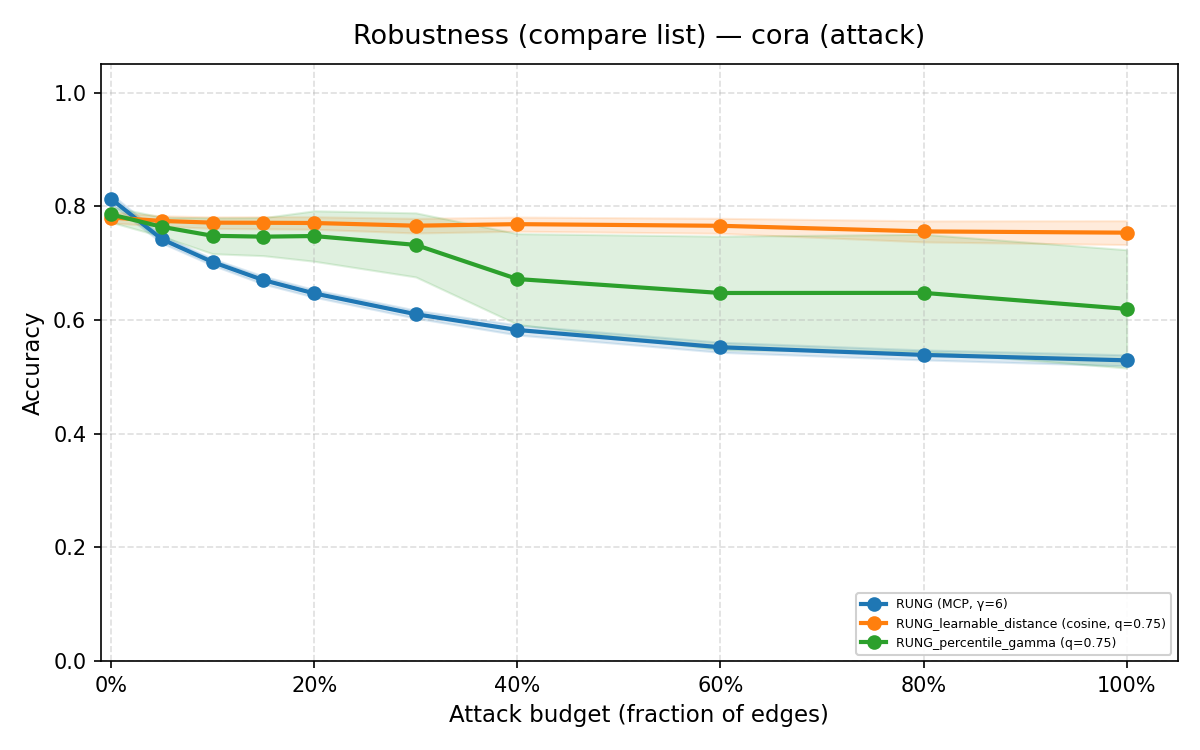
\includegraphics[width=\textwidth]{robustness_cora_compare.png}\\
      \small\textbf{Cora} (Homophily: 0.81)\\
      \vspace{4pt}
      \footnotesize
      RUNG: 81\% $\to$ 53\%\\
      \rungpct{}: maintains 62\%\\
      \rungcos{}: \textbf{75\%} (93\% of clean acc.)
    \end{column}
    \begin{column}{0.33\textwidth}
      \centering
      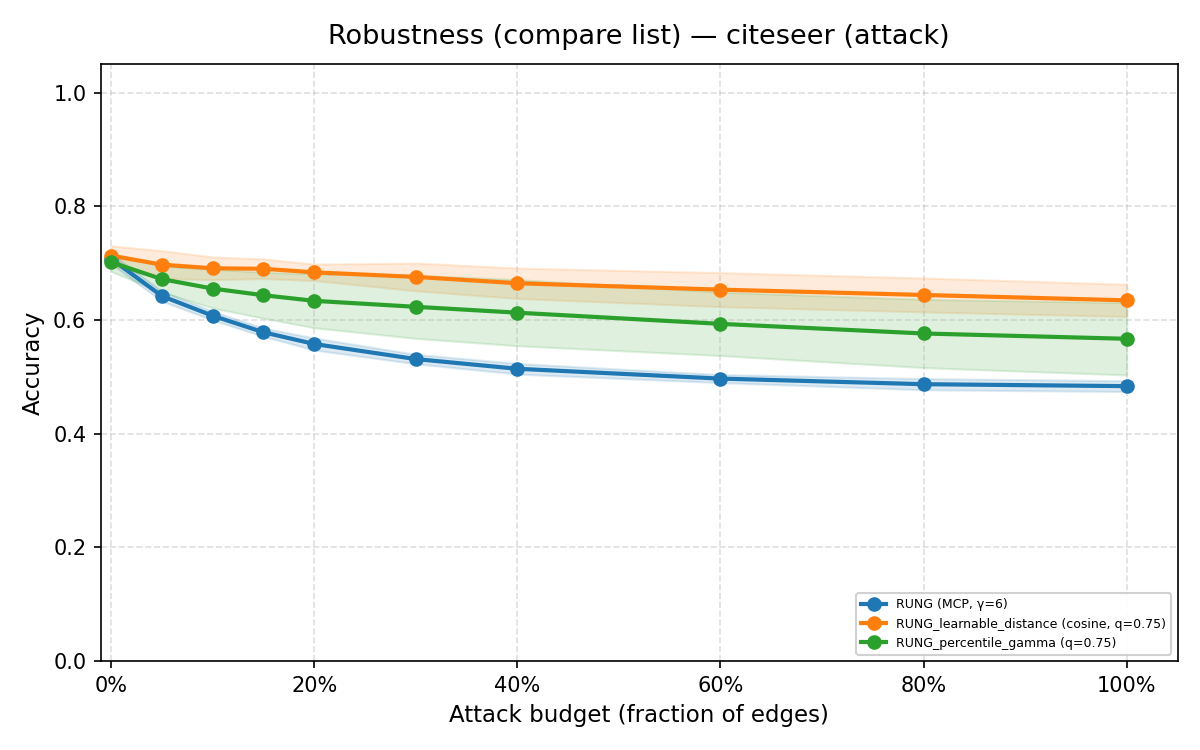
\includegraphics[width=\textwidth]{robustness_citeseer_compare.png}\\
      \small\textbf{Citeseer} (Homophily: 0.74)\\
      \vspace{4pt}
      \footnotesize
      RUNG: drops 22.4 pts\\
      \rungcos{}: degrades only 7.9 pts
    \end{column}
    \begin{column}{0.33\textwidth}
      \centering
      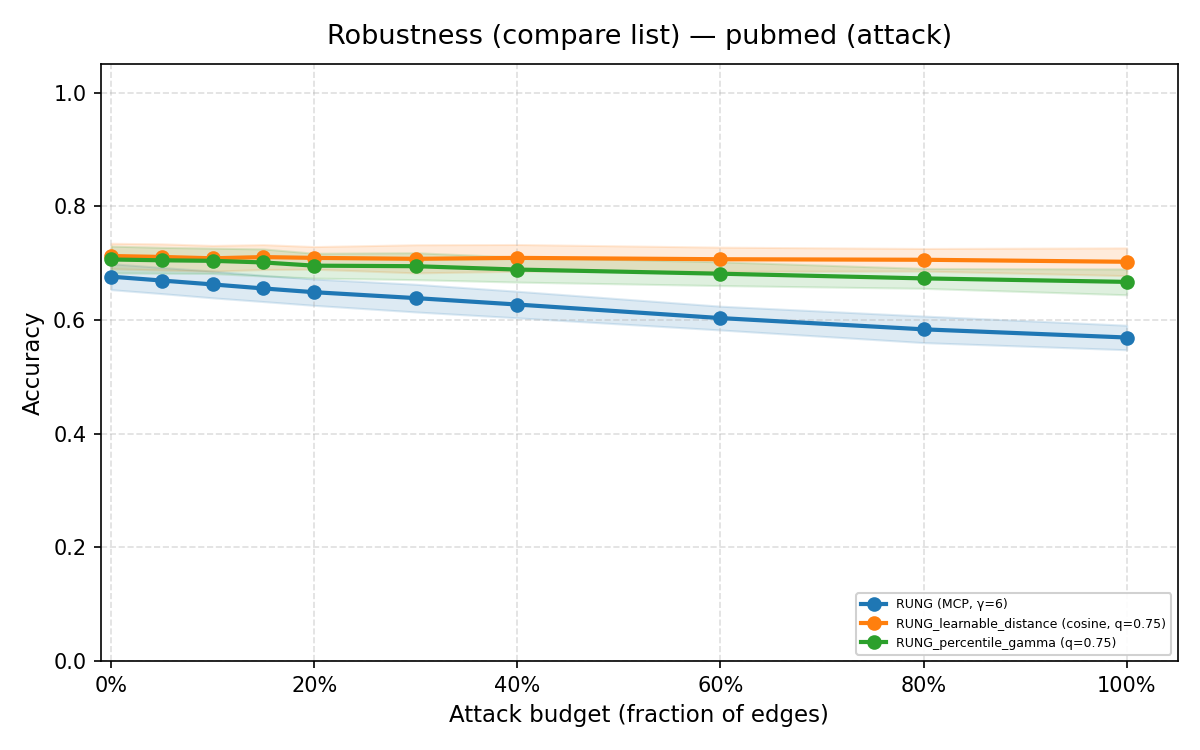
\includegraphics[width=\textwidth]{robustness_pubmed_compare.png}\\
      \small\textbf{Pubmed} (Homophily: 0.80)\\
      \vspace{4pt}
      \footnotesize
      All methods more stable here\\
      \rungcos{}: maintains $\approx$70\% accuracy across all budgets
    \end{column}
  \end{columns}
  \vspace{6pt}
  \begin{block}{Observation}
    On homophilic graphs, all three methods degrade monotonically with increasing budget, but proposed methods maintain substantially higher accuracy at high perturbation budgets.
  \end{block}
\end{frame}

% -----------------------------------------------------------
\begin{frame}{Robustness Degradation Curves --- Heterophilic Graphs}
  \tiny
  \begin{columns}[T]
    \begin{column}{0.33\textwidth}
      \centering
      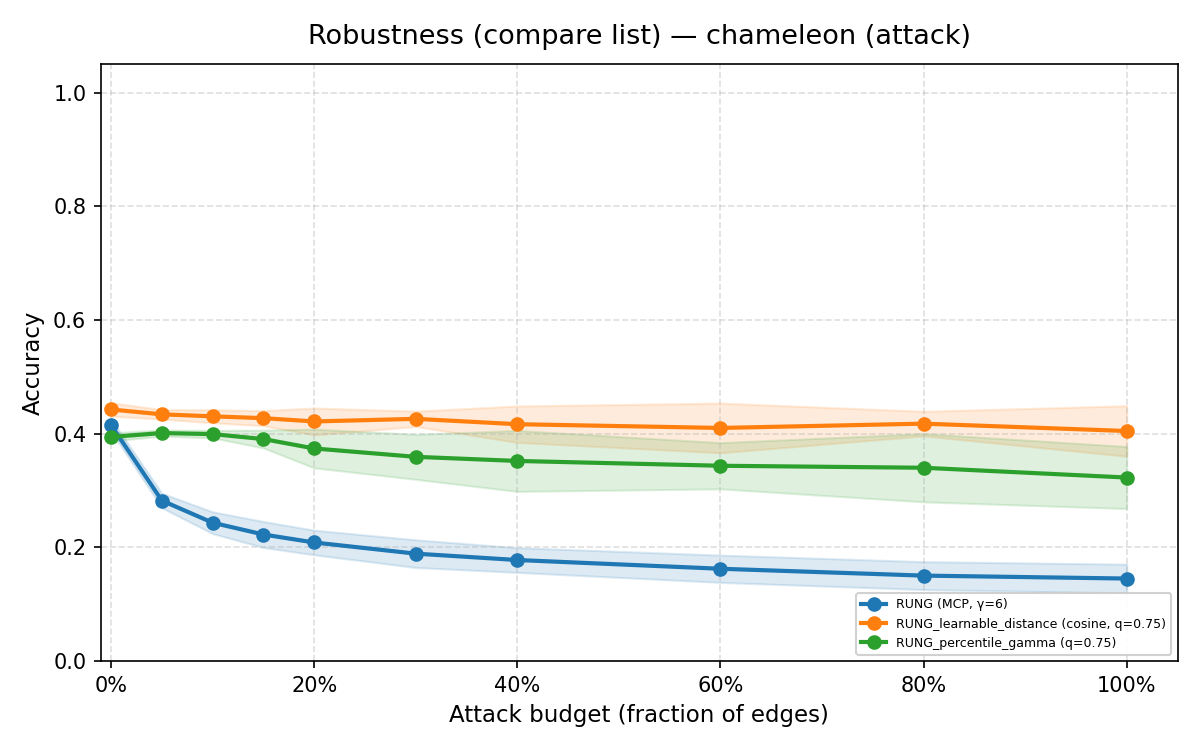
\includegraphics[width=\textwidth]{robustness_chameleon_compare.png}\\
      \small\textbf{Chameleon} (Homophily: 0.23)\\
      \vspace{4pt}
      \footnotesize
      RUNG: \textcolor{red}{41.5\% $\to$ 14.5\%} (catastrophic)\\
      \rungcos{}: \textbf{44.3\% $\to$ 40.5\%}\\
      \textcolor{runggreen}{+25.9 pp absolute improvement}
    \end{column}
    \begin{column}{0.33\textwidth}
      \centering
      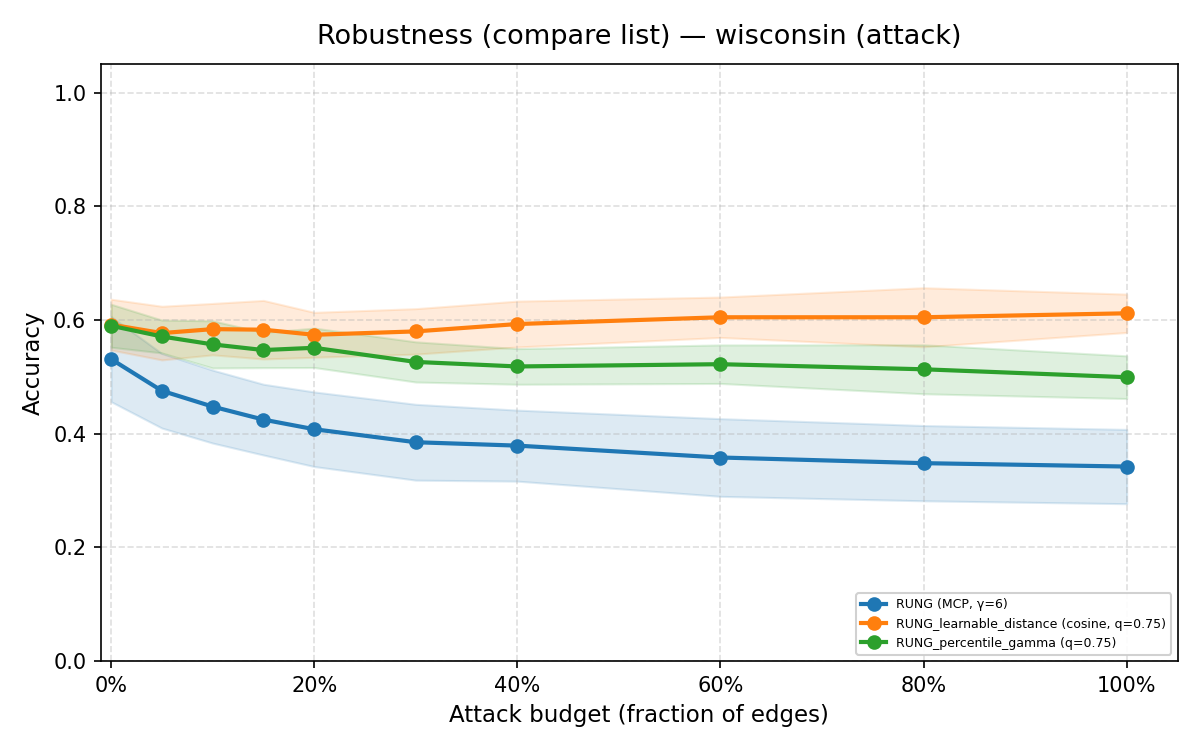
\includegraphics[width=\textwidth]{robustness_wisconsin_compare.png}\\
      \small\textbf{Wisconsin} (Homophily: 0.21)\\
      \vspace{4pt}
      \footnotesize
      RUNG: drops 19 pts\\
      \rungcos{}: \textbf{59\% $\to$ 61\%}\\
      \textcolor{runggreen}{Accuracy \emph{rises} under attack!}
    \end{column}
    \begin{column}{0.33\textwidth}
      \centering
      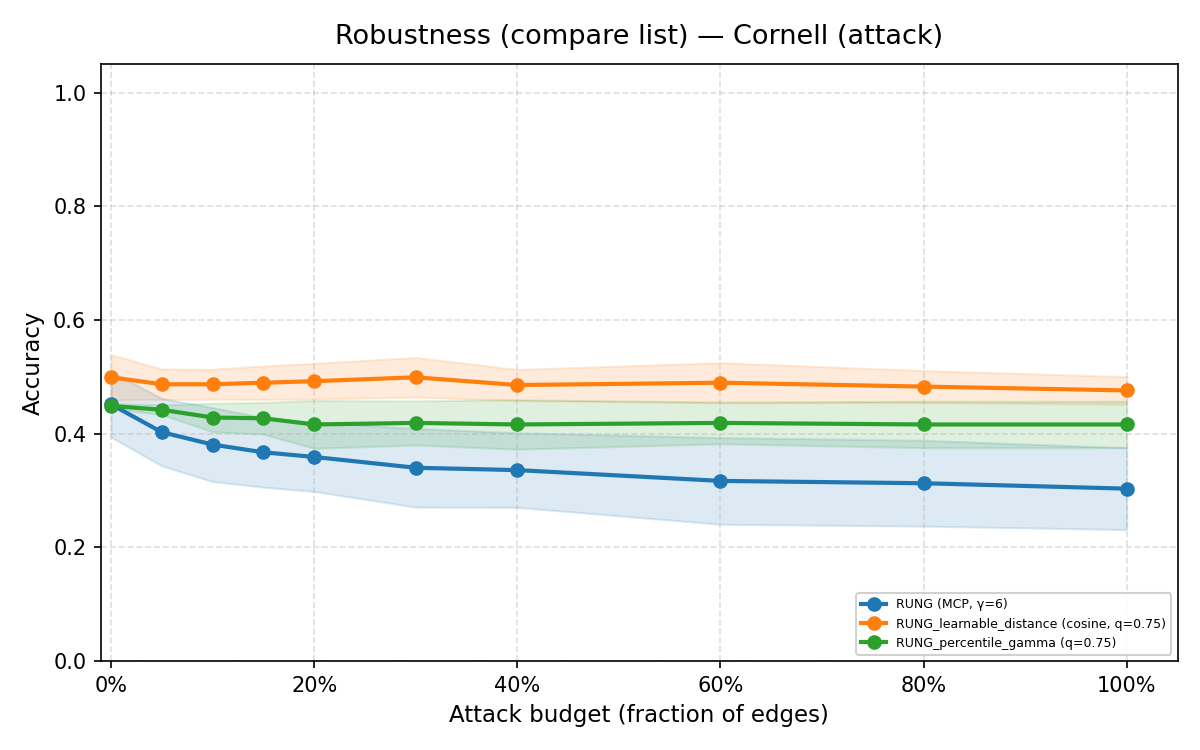
\includegraphics[width=\textwidth]{robustness_cornell_compare.png}\\
      \small\textbf{Cornell} (Homophily: 0.30)\\
      \vspace{4pt}
      \footnotesize
      RUNG: drops 14.8 pts\\
      \rungcos{}: degrades only \textbf{2.3 pts}\\
      \textcolor{runggreen}{+12.5 pp stabilization}
    \end{column}
  \end{columns}
  \vspace{6pt}
  \begin{alertblock}{Key Finding}
    RUNG's curve steepens dramatically in the 20\%--50\% budget range on heterophilic graphs. RUNG-CosineDistance exhibits \textbf{flat degradation}, indicating fundamental architectural alignment with heterophilic structure.
  \end{alertblock}
\end{frame}

% ===========================================================
\section{Analysis \& Discussion}
% ===========================================================

\begin{frame}{Why RUNG Fails on Heterophilic Graphs}
  \tiny
  \begin{columns}[T]
    \begin{column}{0.52\textwidth}
      \begin{alertblock}{RUNG's Flawed Assumption}
        \begin{itemize}
          \item RUNG assumes: \textbf{feature dissimilarity} $\Rightarrow$ adversarial edge
          \item Valid on homophilic graphs (legitimate edges connect similar nodes)
          \item \textbf{Violated on heterophilic graphs} by genuine network structure
        \end{itemize}
      \end{alertblock}
      \vspace{6pt}
      \begin{block}{Chameleon Example (77\% cross-class edges)}
        \begin{itemize}
          \item RUNG's MCP filter assigns zero weight to large-distance edges
          \item Legitimate cross-class edges naturally have large feature distances
          \item RUNG prunes valid edges, weakening graph structure utilization
          \item Attacker's task becomes \emph{easier}: large-distance fake edges are harmless when RUNG is already deleting most high-distance edges
        \end{itemize}
      \end{block}
    \end{column}
    \begin{column}{0.45\textwidth}
      \begin{block}{How Cosine Distance Resolves This}
        \begin{itemize}
          \item Measures \textbf{orientation}, not magnitude
          \item Directional alignment is invariant to feature magnitude
          \item Can distinguish:
          \begin{itemize}
            \item \textcolor{runggreen}{\textbf{Genuine heterophilic edges:}} different directions, legitimately connected (small cosine dist. after learning)
            \item \textcolor{red}{\textbf{Adversarial edges:}} larger cosine dist. after network learns to distinguish
          \end{itemize}
        \end{itemize}
      \end{block}
      \vspace{6pt}
      \begin{block}{Wisconsin Phenomenon}
        RUNG-CosineDistance accuracy \emph{increases} under moderate attack (0\%--60\% budget), suggesting adversarial edges may initially provide additional structural information that the cosine metric effectively filters.
      \end{block}
    \end{column}
  \end{columns}
\end{frame}

% -----------------------------------------------------------
\begin{frame}{Layer-wise Adaptive Threshold Analysis (Cora)}
  \tiny
  \begin{columns}[T]
    \begin{column}{0.48\textwidth}
      \begin{block}{Euclidean Distance Thresholds (Method 1)}
        
        \small
        \begin{tabular}{cc}
          \toprule
          \textbf{Layer $k$} & \textbf{$\gamma^{(k)}$} \\
          \midrule
          0 & 3.6571 \\
          1 & 3.2985 \\
          2 & 3.1846 \\
          3 & 3.1407 \\
          4 & 3.1705 \\
          5 & 3.1592 \\
          6 & 3.1544 \\
          7 & 3.1394 \\
          8 & 3.1445 \\
          9 & 3.1406 \\
          \bottomrule
        \end{tabular}
        \vspace{4pt}\\
        \small Threshold \textbf{decays} from initial to deeper layers as feature smoothing occurs.
      \end{block}
    \end{column}
    \begin{column}{0.48\textwidth}
      \begin{block}{Cosine Distance Statistics (Method 2)}
        \vspace{4pt}
        \tiny
        \begin{tabular}{ccccc}
          \toprule
          \textbf{Layer} & $\gamma^{(k)}$ & \textbf{mean} & \textbf{std} & \textbf{max} \\
          \midrule
          0 & 0.3755 & 0.7520 & 0.3903 & 1.7692 \\
          1 & 0.2494 & 0.7485 & 0.3962 & 1.7407 \\
          2 & 0.2321 & 0.7499 & 0.3999 & 1.7128 \\
          3 & 0.2234 & 0.7524 & 0.4012 & 1.6956 \\
          4 & 0.2209 & 0.7527 & 0.4020 & 1.6956 \\
          5 & 0.2115 & 0.7534 & 0.4022 & 1.6956 \\
          6 & 0.2132 & 0.7536 & 0.4025 & 1.6956 \\
          7 & 0.2065 & 0.7542 & 0.4027 & 1.6956 \\
          8 & 0.2124 & 0.7544 & 0.4029 & 1.6956 \\
          9 & 0.2030 & 0.7547 & 0.4030 & 1.6956 \\
          \bottomrule
        \end{tabular}
        \vspace{4pt}\\
        \small Both $\gamma^{(k)}$ and mean cosine distance decrease with depth, confirming that features become progressively more aligned across layers.
      \end{block}
    \end{column}
  \end{columns}
\end{frame}

% ===========================================================
\section{Limitations \& Future Work}
% ===========================================================

\begin{frame}{Threat Model Constraints: The Feature-Aware Attack}
  \tiny
  \begin{block}{Limitation: Structural-Only Threat Model}
    Current evaluation assumes the attacker can only modify graph topology. A \textbf{fully adaptive adversary with feature perturbations} exposes a fundamental vulnerability.
  \end{block}
  \vspace{4pt}
  \begin{columns}[T]
    \begin{column}{0.52\textwidth}
      \begin{alertblock}{The Feature-Spoofing Attack Mechanism}
        \begin{enumerate}
          \item Attacker observes learned feature representation of target node $v_\text{target}$
          \item Sets adversarial node feature $\mathbf{x}_\text{adv} \approx \mathbf{x}_\text{target}$
          \item Adds edge connecting them
          \item Both Euclidean and cosine distance $\to 0$
          \item QN-IRLS assigns \textbf{maximum weight} to the adversarial edge
        \end{enumerate}
        If $\delta_f$ large enough: $W^{(k)}_\text{adv,target} = \text{MCP}(y^{(k)} \approx 0) \to 1$
      \end{alertblock}
    \end{column}
    \begin{column}{0.45\textwidth}
      \begin{block}{Why Practical Constraints Limit This Attack}
        \begin{itemize}
          \item \textbf{Citation networks:} Cannot change paper title/abstract without detectable inconsistencies --- $\approx 0.3\%$ feature budget
          \item \textbf{Social networks:} Fake account creation dates, follower counts, posting history trigger detection systems
          \item \textbf{Biological networks:} Cannot synthesize proteins with arbitrary sequences
        \end{itemize}
        \vspace{4pt}
        Small $\delta_f < 0.1$: distance remains large, defense holds.\\
        Large $\delta_f > 0.3$: defense \textbf{collapses entirely}.
      \end{block}
    \end{column}
  \end{columns}
\end{frame}

% -----------------------------------------------------------
\begin{frame}{Future Work Directions}
  \tiny
  \begin{columns}[T]
    \begin{column}{0.48\textwidth}
      \begin{block}{1. Feature-Aware Adversarial Attacks}
        Implement joint edge-and-feature attack:
        \[
          \mathcal{A}_\text{joint} = \{(\tilde{A}, \tilde{X}) : \Delta_\text{edge} + \Delta_\text{feature} \leq B\}
        \]
        Craft specifically to minimize intended edge's cosine distance while keeping nodes dissimilar in feature content.
      \end{block}
      \vspace{6pt}
      \begin{block}{2. Theoretical Robustness Analysis}
        Analyze whether MCP-based estimators applied to cosine distances maintain the \textbf{unbiasedness property} from the original RUNG analysis. Extend Hou et al.\ [NeurIPS 2024] to non-Euclidean metrics.
      \end{block}
    \end{column}
    \begin{column}{0.48\textwidth}
      \begin{block}{3. Scalability Improvements}
        \begin{itemize}
          \item Distributed quantile computation and sparse cosine distance kernels for multi-GPU inference
          \item Benchmark on large-scale graphs (Ogbn-Arxiv: 1.63M nodes, 40.9M edges)
          \item Current evaluation limited to moderate scale (Wisconsin: 251 nodes; Pubmed: 19,717 nodes)
        \end{itemize}
      \end{block}
      \vspace{6pt}
      \begin{block}{4. Learnable Distance Metrics Beyond Cosine}
        Extend to bilinear and projection-based metrics with trainable parameters for further geometry adaptation to specific graph structures.
      \end{block}
    \end{column}
  \end{columns}
\end{frame}

% ===========================================================
\section{Conclusion}
% ===========================================================

\begin{frame}{Conclusion}
  \tiny
  \begin{block}{Summary of Contributions}
    Two complementary enhancements to RUNG (NeurIPS 2024 state-of-the-art):
    \begin{itemize}
      \item \textbf{Method 1 --- Adaptive Percentile-based Thresholding:} Layer-wise pruning thresholds from empirical edge-distance quantiles; no learnable parameters; automatic scale tracking
      \item \textbf{Method 2 --- Learnable Cosine-Distance Modules:} Angle-based distance metric; gradient-driven feature learning; optimal subspace discovery for legitimate vs.\ adversarial edge discrimination
    \end{itemize}
  \end{block}
  \vspace{4pt}
  \begin{columns}[T]
    \begin{column}{0.48\textwidth}
      \begin{block}{Key Findings}
        \begin{itemize}
          \item \textbf{Homophilic graphs:} +22.5 pp (Cora), +15.1 pp (Citeseer), +13.3 pp (Pubmed) at maximum budget
          \item \textbf{Heterophilic graphs:} RUNG's 27-pt degradation on Chameleon reduced to 3.8 pts; Wisconsin accuracy \emph{rises} under attack
          \item Both methods outperform RUNG on \textbf{all six datasets}
        \end{itemize}
      \end{block}
    \end{column}
    \begin{column}{0.48\textwidth}
      \begin{alertblock}{Open Problems}
        \begin{itemize}
          \item No formal theoretical guarantees for adaptive thresholding or cosine geometry
          \item Feature-aware adversary can bypass distance-based defenses
          \item Large-scale evaluation not yet conducted
          \item These gaps represent important future research directions
        \end{itemize}
      \end{alertblock}
    \end{column}
  \end{columns}
  \vspace{6pt}
  \centering
  \textit{Heterophilic-robust graph learning is achievable through adaptive per-layer thresholding combined with learnable angle-based distance metrics.}
\end{frame}

% -----------------------------------------------------------
\begin{frame}{References}
  \tiny
  \begin{enumerate}
    \item Hou et al. \textit{Robust Graph Neural Networks via Unbiased Aggregation.} NeurIPS 2024.
    \item Li et al. \textit{Towards Robust Graph Neural Networks.} IEEE ICDM 2020.
    \item Luan et al. \textit{Towards Deeper Graph Neural Networks with Differentially Private Learning.} ICML 2022.
    \item Sun et al. \textit{Adversarial Attacks on Graphs: Deep Insights and Best Practices.} IJCAI 2021.
    \item Tam et al. \textit{Defending Against Adversarial Attacks by Reconstruction.} NeurIPS 2021.
    \item Xu et al. \textit{Topology Attack and Defense for Graph Neural Networks: An Optimization Perspective.} IJCAI 2019.
    \item Yan et al. \textit{Heterophilic Graph Neural Network.} NeurIPS 2021.
    \item Zhang. \textit{Nearly Unbiased Variable Selection Under Minimax Concave Penalty.} Annals of Statistics 2010.
    \item Zhu et al. \textit{Beyond Homophily in Graph Neural Networks.} NeurIPS 2020.
    \item Zhu et al. \textit{GNNGuard: Defending GNNs against Adversarial Attacks.} NeurIPS 2020.
    \item Zugner et al. \textit{Adversarial Attacks on Neural Networks for Graph Data.} KDD 2018.
    \item Zugner \& Günnemann. \textit{Certifiable Robustness and Robust Training of GCNs.} KDD 2019.
  \end{enumerate}
\end{frame}

\end{document}